Knihovna \texttt{tnums} nyní implementuje racionální čísla, Ludolfovo číslo, aditivní a multiplikativní operace. Dobrým zdrojem dalších iracionálních čísel, jak jsem napsal již v~podkapitole \ref{funkce_cisel}, jsou matematické funkce. V této kapitole zavedeme exponenciálu, logaritmus, goniometrické funkce a mocninné operace.

\subsection{Aproximace funkcí}
Stejně jako matematické funkce berou reálné číslo a vrací reálné číslo, musejí tnumovské funkce přijímat tnumy a vracet tnumy. Nástroj, který poskytuje vyčíslování funkcí i odhad chyby vyčíslení se nazývá Taylorův polynom (TP). Ten z bodu $a$, kterému říkáme počátek, odhaduje průběh funkce pomocí polynomů určitého stupně. Pro funkci $f$ budu TP stupně $n$ se středem v $a$ značit $T^{f,a}_n$. K implementaci TP využijeme funkci faktoriálu přirozeného čísla.

\begin{lispcode}{\texttt{factorial}}{Funkce pro výpočet faktoriálu v iterativní verzi, kvůli přetékání zásobníku při velkých vstupech není použita rekurze}
(\textcolor{funkcionalni}{defun} \textcolor{pojmenovan}{factorial} (n)
  (\textcolor{vedlejsi}{let} ((result 1))
    (\textcolor{funkcionalni}{loop} \textcolor{obarvi}{for} i \textcolor{obarvi}{from} n \textcolor{obarvi}{downto} 1
          \textcolor{obarvi}{do} (\textcolor{vedlejsi}{setf} result (\textcolor{matematicke}{*} result i)))
    result))
\end{lispcode}

TP počítá aproximaci funkce $f$ v bodě $x$ následovně: nejjednodušší je vzít funkci $T^{f,a}_0(x) = f(a)$. Přesněji funkci v daném bodě reprezentuje TP prvního stupně -- přímka, která se dotýká grafu funkce $f$ v bodě $a$: $T^{f,a}_1(x) = f(a)+f'(a)(x-a)$. Tato aproximace nebere v úvahu jen hodnotu funkce $f$ v bodě $a$, ale i její první derivaci -- směr, kam se z počátku pohybuje. Ještě přesnější je TP druhého stupně -- parabola přimknutá k grafu funkce $f$ v bodě $a$: $T^{f,a}_2(x) = f(a)+f'(a)(x-a)+\frac{f''(a)}{2}(x-a)^2$. Teď už TP zohledňuje funkční hodnotu, směr křivky i konvexnost. Ještě lepší je použít $T^{f,a}_3(x)=f(a)+f'(a)(x-a)+\frac{f''(a)}{2}(x-a)^2+\frac{f'''(a)}{6}(x-a)^3$ a tak dále \cite{MTTP}.

\begin{remind}[Taylorova a Maclaurinova řada]
Kdybychom takto postupovali donekonečna -- $\lim_{n\to\infty}T^{f,a}_n(x)$ -- dostali bychom Taylorovu řadu z definice \ref{def:taymac_rada}. Pro $a=0$ pak Taylorovu řadu nazýváme řadou Maclaurinovou.
\end{remind}

Pokud Taylorovy zbytky konvergují k nule, lze Taylorovou řadou $T_\infty^{f,a}$ nahradit funkci $f$ \cite{ZDVNNR}. My pro výpočty s libovolnou přesností navíc potřebujeme velikosti zbytků odhadovat.

\begin{fact}[Taylorova věta \cite{TMA:Calculus}]
Nechť $f$ má spojité derivace až do řádu $n+1$ na libovolném intervalu obsahujícím $a$. Pak pro každé $x$ z tohoto intervalu máme Taylorův vzorec
\begin{equation}
f(x) = T_n^{f,a}(x) + R_n^{f,a}(x)\text{, kde}
\end{equation}
\begin{equation}\label{TP}
T_n^{f,a}(x) = \sum_{i=0}^{n}\frac{f^{(i)}(a)}{i!}(x-a)^i\text{~a~také}
\end{equation}
\begin{equation}\label{integralnitvar}
R_n^{f,a}(x)=\int_a^x\frac{(x-t)^n}{n!}f^{(n+1)}(t)dt.
\end{equation}
Navíc existuje číslo $\xi$, z intervalu s krajními body $x$ a $a$ takové, že
\begin{equation}\label{lagrangeuvtvar}
R_n^{f,a}(x)=\frac{f^{(n+1)}(\xi)}{(n+1)!}(x-a)^{n+1}.
\end{equation}
Pro důkaz vizte kapitolu 7.5 v \cite{TMA:Calculus}.
\end{fact}

Součet v rovnici \eqref{TP} nazýváme Taylorův polynom funkce $f$ stupně $n$ v bodě $a$, $R_n^{f,a}(x)$ nazýváme $n$-tým Taylorovým zbytkem. Vyjádření \eqref{integralnitvar} pak říkáme \textit{integrální tvar} zbytku a \eqref{lagrangeuvtvar} je Lagrangeův tvar zbytku \cite{MTTP}.

Takto vyjádřené zbytky můžeme zhora omezovat, podobně jako tomu bylo u geometrické řady. 

\subsection{Exponenciála}
Exponenciála je funkce s předpisem $\mathrm{exp}(x) = e^x$ kde $e$ je tzv. \textit{Eulerovo číslo} definované jako $e=\lim_{n\to\infty}\left(1+\frac{1}{n}\right)^n$ \cite{EPJVMAI}. Eulerovo číslo je transcendentní konstanta, je též základem přirozeného logaritmu. Exponenciála je z tohoto důvodu nazývána též přirozená mocnina. Platí: $\frac{d}{dx}\mathrm{exp}(x)=\mathrm{exp}(x),D(\mathrm{exp})=\mathbb{R},H(\mathrm{exp})=\mathbb{R}^+$.

\begin{myremark}{Značení exponenciály}
Ačkoli to působí nezvykle, značím exponenciálu jako $\mathrm{exp}$, protože potřebuji vyjadřovat i název funkce, nikoli jen její hodnotu a pro to se nehodí obvyklejší zápis pomocí $e^x$. Navíc zápis $\mathrm{exp}(x)$ pro závisle proměnnou lépe vyjadřuje, že je exponenciála funkcí.
\end{myremark}

\subsubsection{Exponenciála čísla}

\begin{fact}[Exponenciála jako Maclaurinova řada \cite{ZDVNNR}]\label{vet:exp_jako_rada}
Funkci $\mathrm{exp}$ lze vyjádřit jako Maclaurinovu řadu ve tvaru
\begin{equation}
\mathrm{exp}(x) = \underset{i \in \mathbb{N}}{\sum} \frac{x^i}{i!} = \frac{1}{1} + \frac{x}{1} + \frac{x^2}{2!} + \frac{x^3}{3!} + \ldots
\end{equation}
\end{fact}

Zbytek této řady vyjádřený v Lagrangeově tvaru je pro neznámé $\xi$ v intervalu s krajními body $0$ a $x$ roven
\begin{equation}
R_n^{exp, 0}(x) = \frac{e^\xi}{(n+1)!}x^{n+1}.
\end{equation}

Exponenciála je funkce rostoucí a $e<2.72$, a platí tedy
\begin{equation}
(\forall\xi\in (0,x))(\mathrm{exp}(\xi)<\mathrm{exp}(x) < 2.72^x).
\end{equation}
Získáváme odhad chyby aproximace exponenciály pomocí TP.
\begin{fact}[Omezení Taylorova zbytku exponenciály]
Pro $x\in\mathbb{R}$ platí
\begin{equation}
|R_n^{exp, 0}(x)| = \left|\mathrm{exp}(x)- \sum_{i=0}^n \frac{x^i}{i!}\right| \leq \left| \frac{2.72^x}{(n+1)!}x^{n+1} \right|.
\end{equation}
\end{fact}

\begin{consequence}[Exponenciála numu]
Nechť $x\in\mathbb{Q}$ a funkce $\tnum{}(x)$ má předpis
\begin{equation}
\tnum{}(x)(\varepsilon)=\left[\begin{array}{l}\mathrm{1.~}\text{Najdi~nejmenší~}n\in\mathbb{N}^+\text{~tak,~aby~}\left|\frac{2.72^x}{(n+1)!}x^{n+1}\right| \leq \varepsilon;\\
\mathrm{2.~}\text{Vrať~}\sum_{i=0}^n \frac{x^i}{i!},\end{array}\right.
\end{equation}
pak $\tnum{}(x)\in\Tnum{\mathrm{exp}(x)},x\in\mathbb{Q}$.
\begin{proof}
Existence čísla $n$ je zřejmá z definice limity posloupnosti a z toho, že limita podílu polynomu a faktoriálu je rovna nule.

Dále protože $\mathrm{exp}(x) = T^{exp, 0}_n(x)+R^{exp, 0}_n(x)$, lze psát
\begin{equation}
T^{exp, 0}_n(x) \in [\mathrm{exp}(x) - |R^{exp, 0}_n(x)|, \mathrm{exp}(x) + |R^{exp, 0}_n(x)|],
\end{equation}
přičemž dle předchozího faktu platí
\begin{equation}
T^{exp, 0}_n(x) \in \left[\mathrm{exp}(x) - \left| \frac{2.72^x}{(n+1)!}x^{n+1} \right|, \mathrm{exp}(x) + \left| \frac{2.72^x}{(n+1)!}x^{n+1} \right|\right]
\end{equation}
a z kroku 1. pak
\begin{equation}
T^{exp, 0}_n(x) \in [\mathrm{exp}(x) - \varepsilon, \mathrm{exp}(x) + \varepsilon].
\end{equation}
\end{proof}
\end{consequence}

Při implementaci stačí jen iterovat přes $n$ a po cestě sčítat řadu, dokud nebude zbytek menší než $\varepsilon$. Stejný přístup jsme viděli již u Ludolfova čísla.

\begin{lispcode}{\texttt{num-exp}}{Funkce exponenciálu numu}
(\textcolor{funkcionalni}{defun} \textcolor{pojmenovan}{num-exp} (num eps)
  (\textcolor{vedlejsi}{let} ((above (\textcolor{moje}{rat-expt} 272/100 num)) (result 0))
    (\textcolor{funkcionalni}{loop} \textcolor{obarvi}{for} n \textcolor{obarvi}{from} 0
          \textcolor{obarvi}{for} nfact = (\textcolor{moje}{factorial} n)
          \textcolor{obarvi}{for} xpown = (\textcolor{matematicke}{expt} num n)
          \textcolor{obarvi}{do} (\textcolor{vedlejsi}{incf} result (\textcolor{matematicke}{/} xpown nfact))
          \textcolor{obarvi}{until} (\textcolor{matematicke}{<=} (\textcolor{matematicke}{/} (\textcolor{matematicke}{*} above xpown) nfact) eps)
          \textcolor{obarvi}{finally} (\textcolor{funkcionalni}{return} result))))
\end{lispcode}

\begin{myremarkbez}{Eulerovo číslo jako exponenciála čísla jedna}
Protože $e = e^1$, lze přidat i tnum Eulerova čísla.
\begin{lispcode}{\texttt{tnum-e}}{Funkce pro tnum Eulerova čísla\hfill$\blacksquare$}
(\textcolor{funkcionalni}{defun} \textcolor{pojmenovan}{tnum-e} ()
  (\textcolor{funkcionalni}{lambda} (eps)
    (\textcolor{moje}{num-exp} 1 eps)))
\end{lispcode}
\end{myremarkbez}

Do knihovny přibyl tnum exponenciály čísla, lze tedy napsat
\begin{equation}
\texttt{(num-exp } q \texttt{)}\in\Tnum{\mathrm{exp}(q)}, q\in\mathbb{Q}.
\end{equation}

\subsubsection{Exponenciála tnumu}
I při implementaci exponenciály tnumu vyvstává rozdíl mezi přístupem k racionálním číslům a číslům rekurzivním.

Víme, že $(\forall\tnum{x}\in\Tnum{x})(\txe \in [x-\varepsilon,x+\varepsilon])$. Na Obrázku \ref{fig:exp1} je znázorněno, že $[\mathrm{exp}(x)-\varepsilon,\mathrm{exp}(x)+\varepsilon]\neq[\mathrm{exp}(x-\varepsilon),\mathrm{exp}(x+\varepsilon)]$.

\begin{myfigure}{}
\caption{Obraz přesnosti po průchodu exponenciálou}
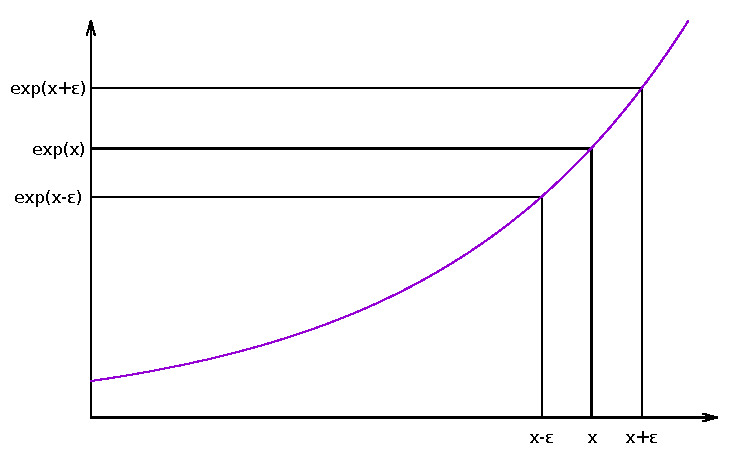
\includegraphics[width=\linewidth]{graphics/exp1.pdf}\label{fig:exp1}
Interval $[x-\varepsilon,x+\varepsilon]$ se nezobrazí na $[e^x-\varepsilon,e^x+\varepsilon]$. Tím pádem $\tnum{\mathrm{exp}(\txe)}\not\in\Tnum{\mathrm{exp}(x)},x\in\mathbb{R}$.
\end{myfigure}

Dále na Obrázku \ref{fig:exp2} vidíme, že abychom dodrželi přesnost závisle proměnné, musíme manipulovat s přesností nezávisle proměnné.\begin{myfigure}{}
\caption{Vzor přesnosti před průchodem exponenciálou}
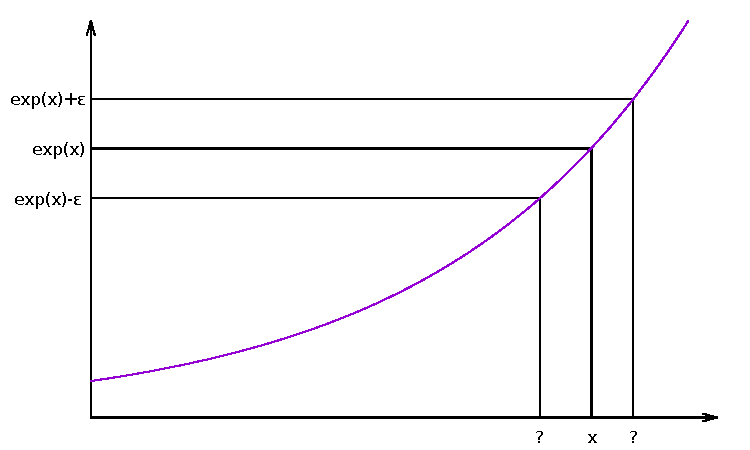
\includegraphics[width=\linewidth]{graphics/exp2.pdf}\label{fig:exp2}
Hledáme, jaké okolí bodu $x$ se zobrazí na $\varepsilon$-okolí bodu $e^x$.
\end{myfigure} Závislost můžeme pospat rovnicí
\begin{equation}\label{invpresexp}
\mathrm{exp}(x)+\varepsilon=\mathrm{exp}(x+w),
\end{equation}
kde hledaná neznámá je $w$. Ilustraci tohoto vztahu najdeme na Obrázku \ref{fig:exp6}.

\begin{myfigure}{}
\caption{Zobrazení neznámé $w$}
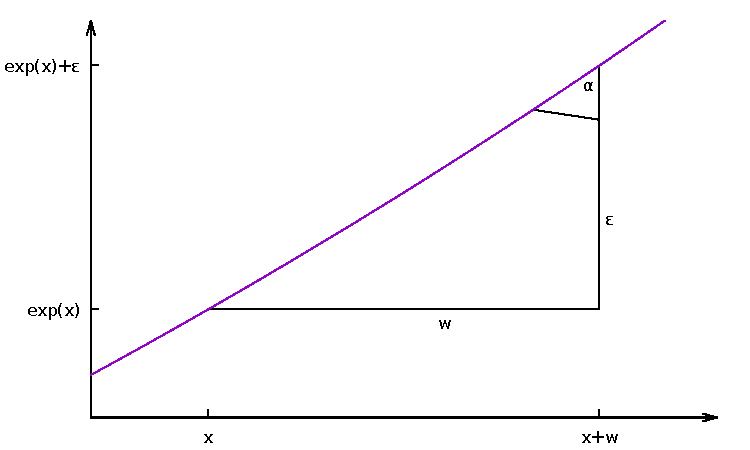
\includegraphics[width=\linewidth]{graphics/exp6.pdf}\label{fig:exp6}
Neznámou $w$ lze zobrazit jako jednu z odvěsen, druhá je $\varepsilon$. Fialová čára není přepona, ale exponenciála. Protože se ale $\varepsilon$ může neomezeně zmenšovat, exponenciála se k přeponě blíží.
\end{myfigure}

Je třeba najít vztah mezi $w$ a $\varepsilon$. Pro úhel $\alpha$ při vrcholu $W$ platí $\mathrm{ctan}(\alpha) = \frac{\varepsilon}{w}$. Tedy
\begin{equation}
w = \frac{\varepsilon}{\mathrm{ctan}(\alpha)} = \frac{\varepsilon}{\mathrm{tan}(\frac{\pi}{2}-\alpha)} = \frac{\varepsilon}{exp(x+w)}.
\end{equation}

Poslední úprava je přepis skutečnosti, že tangens je v tomto bodě roven derivaci a derivace exponenciály je exponenciála. Vychází rekurzivní vztah pro $w$, po jehož dosazení do vztahu \eqref{invpresexp} dostáváme
\begin{equation}\label{rekpresexp}
\mathrm{exp}(x)+\varepsilon=\mathrm{exp}\left(x+\frac{\varepsilon}{\mathrm{exp}\left(x+\frac{\varepsilon}{\mathrm{exp}(x+\ldots)}\right)}\right).
\end{equation}

Podobným způsobem lze odvodit i vztah pro opačný kraj okolí a to
\begin{equation}\label{rekpresexp2}
\mathrm{exp}(x)-\varepsilon=\mathrm{exp}\left(x-\frac{\varepsilon}{\mathrm{exp}\left(x-\frac{\varepsilon}{\mathrm{exp}(x-\ldots)}\right)}\right).
\end{equation}

\begin{myremarkbez}{Obecnější přesnost vzoru}
Právě odvozený vztah není specifický jen pro exponenciálu, uveďme si obecnější znění.
\begin{fact}[O přesnosti závislé proměnné]\label{lem:presprom}Nechť $f$ je neklesající funkce spojitá na celém definičním oboru, pak
\begin{equation}\label{eq:presprom}
\begin{aligned}
[f(x)-\varepsilon , f(x)+\varepsilon]&=[f(x-v),f(x+w)],\\\text{~kde~}v&=f\left(x-\frac{\varepsilon}{f^{'}(x-v)}\right),w=f\left(x+\frac{\varepsilon}{f^{'}(x+w)}\right).\mathrm{~~~~~\hfill}\blacksquare
\end{aligned}
\end{equation}
\end{fact}
\end{myremarkbez}

Z výše uvedených vztahů je jasné, že při implementaci budeme hledat pevný bod. Proto si zavedeme tzv. \textit{precizní iterátor}.

\begin{definition}[Precizní iterátor exponenciály]
Nechť $\tnum{\mathrm{exp}(q)}\in\Tnum{\mathrm{exp}(q)},q\in\mathbb{Q}$. Pak definujme následující posloupnost:
\begin{equation}
\left[\tnum{x}\right]_0^{\mathrm{exp},\varepsilon}=\tnum{\mathrm{exp}(\txe)}(\varepsilon),
\end{equation}
\begin{equation}
\left[ \tnum{x}\right]_{n+1}^{\mathrm{exp},\varepsilon}=\tnum{\mathrm{exp}\left(\tnum{x}\left(\frac{\varepsilon}{\left|\left[ \tnum{x}\right]_n^{\mathrm{exp},\varepsilon}\right|+\varepsilon}\right)\right)}(\varepsilon)
\end{equation}
a pokud existuje $m$ tak, že
\begin{equation}
\left[\tnum{x}\right]_m^{\mathrm{exp},\varepsilon} = \left[\tnum{x}\right]_{m+1}^{\mathrm{exp},\varepsilon},
\end{equation}
pak klademe
\begin{equation}
\left[\tnum{x} \right]_\infty^{\mathrm{exp},\varepsilon} := \left[\tnum{x}\right]_m^{\mathrm{exp},\varepsilon}.
\end{equation}
\end{definition}

\begin{consequence}[Exponenciála tnumu]\label{dusl:expotnumu}
Nechť $\tnum{x}\in\Tnum{x},x\in\mathbb{R}$ a funkce $\tnum{}(\tnum{x})$ má předpis
\begin{equation}
\tnum{}(\tnum{x})(\varepsilon)=\left[\tnum{x}\right]_\infty^{exp,\varepsilon},
\end{equation}
pak $\tnum{}(\tnum{x})\in\Tnum{\mathrm{exp}(x)},x\in\mathbb{R}$.
\begin{proof}
Vychází přímo ze vztahů \eqref{rekpresexp} a \eqref{rekpresexp2}.
\end{proof}
\end{consequence}

\begin{lispcode}{\texttt{tnum-exp}}{Funkce pro exponenciálu tnumu}
(\textcolor{funkcionalni}{defun} \textcolor{pojmenovan}{tnum-exp} (tnum)
  (\textcolor{funkcionalni}{lambda} (eps)
    (\textcolor{funkcionalni}{loop} \textcolor{obarvi}{for} i \textcolor{obarvi}{from} 0
          \textcolor{obarvi}{for} num = (\textcolor{funkcionalni}{if} (\textcolor{funkcionalni}{zerop} i) (\textcolor{moje}{tnum-to-num} tnum eps) new)
          \textcolor{obarvi}{for} new = (\textcolor{funkcionalni}{if} (\textcolor{funkcionalni}{zerop} i) 1
                      (\textcolor{funkcionalni}{if} (\textcolor{matematicke}{>} expnum 1)
                          (\textcolor{moje}{tnum-to-num} tnum (\textcolor{matematicke}{/} eps 
                                               (\textcolor{matematicke}{+} expnum eps)))
                        num))
          \textcolor{obarvi}{for} expnum = (\textcolor{moje}{num-exp} num eps)
          \textcolor{obarvi}{until} (\textcolor{matematicke}{=} num new) 
          \textcolor{obarvi}{finally} (\textcolor{funkcionalni}{return} expnum))))
\end{lispcode}

\subsection{Goniometrické}
Goniometrické funkce jsou reálné funkce reálné proměnné. Platí $\frac{d}{dx}\mathrm{sin}(x) = \mathrm{cos}(x)$, $\frac{d}{dx}\mathrm{cos}(x) = -\mathrm{sin}(x)$ a $H(\mathrm{sin}) = [-1,1] = H(\mathrm{cos})$.

\subsubsection{Sinus}
\begin{fact}[Sinus jako Maclaurinova řada \cite{ZDVNNR}]\label{vet:sin_jako_rada}
Funkci $\mathrm{sin}$ lze vyjádřit jako Maclaurinovu řadu ve tvaru
\begin{equation}
\mathrm{sin}(x) =\sum_{i \in \mathbb{N}} (-1)^i \frac{x^{2i+1}}{(2i+1)!} =\frac{x}{1} - \frac{x^3}{3!} + \frac{x^5}{5!} - \frac{x^7}{7!} + \ldots
\end{equation}
\end{fact}

Dále protože jsou funkční hodnoty všech možných derivací v intervalu $[-1,1]$, lze Lagrangeův tvar zbytku vyjádřit bez znaménka, a pak díky Taylorově větě platí
\begin{equation}
\left|\mathcal{R}^{sin, 0}_n(x)\right|\leq\left|\frac{x^{2n+1+1}}{(2n+1+1)!}\right|=\left|\frac{x^{2n+2}}{(2n+2)!}\right|.
\end{equation}

\begin{consequence}[Sinus numu]
Nechť $x\in\mathbb{Q}$ a funkce $\tnum{}(x)$ má předpis
\begin{equation}
\tnum{}(x)(\varepsilon)=\left[\begin{array}{l}\mathrm{1.~}\text{Najdi~nejmenší~}n\in\mathbb{N}^+\text{~tak,~aby~}\left|\frac{x^{2n+2}}{(2n+2)!}\right| \leq \varepsilon;\\
\mathrm{2.~}\text{Vrať~}\sum_{i=0}^n (-1)^i \frac{x^{2i+1}}{(2i+1)!},\end{array}\right.
\end{equation}
pak $\tnum{}(x)\in\Tnum{\mathrm{sin}(x)},x\in\mathbb{Q}$.
\begin{proof}
Jde opět o polynom nad faktoriálem, proto je vidět limita i existence $n$. Z omezení $R^{\mathrm{sin}, 0}_n$ je zřejmé, že pokud platí $T^{\mathrm{sin}, 0}_n\in[\mathrm{sin}(x)-|R^{\mathrm{sin}, 0}_n|,\mathrm{sin}(x)+|R^{\mathrm{sin}, 0}_n|]$, pak musí platit i $T^{\mathrm{sin}, 0}_n\in[\mathrm{sin}(x)-|\frac{x^{2n+2}}{(2n+2)!}|,\mathrm{sin}(x)+|\frac{x^{2n+2}}{(2n+2)!}|]$, a tudíž $T^{\mathrm{sin}, 0}_n\in[\mathrm{sin}(x)-\varepsilon,\mathrm{sin}(x)+\varepsilon]$.
\end{proof}
\end{consequence}

\begin{lispcode}{\texttt{num-sin}}{Funkce pro sinus čísla}
(\textcolor{funkcionalni}{defun} \textcolor{pojmenovan}{num-sin} (x eps)
  (\textcolor{vedlejsi}{let} ((result 0))
    (\textcolor{funkcionalni}{loop} \textcolor{obarvi}{for} n \textcolor{obarvi}{from} 0
          \textcolor{obarvi}{for} 2n+1 = (\textcolor{matematicke}{1+} (\textcolor{matematicke}{*} 2 n))
          \textcolor{obarvi}{do} (\textcolor{vedlejsi}{incf} result
                   (\textcolor{matematicke}{/} (\textcolor{moje}{rat-expt} x 2n+1)
                      (\textcolor{moje}{factorial} 2n+1) (\textcolor{matematicke}{expt} -1 n)))
          \textcolor{obarvi}{until} (\textcolor{matematicke}{<} (\textcolor{matematicke}{abs} (\textcolor{matematicke}{/} (\textcolor{moje}{rat-expt} x (\textcolor{matematicke}{1+} 2n+1))
                           (\textcolor{moje}{factorial} (\textcolor{matematicke}{1+} 2n+1))))
                   eps)
          \textcolor{obarvi}{finally} (\textcolor{funkcionalni}{return} result))))
\end{lispcode}

Protože derivace sinu je kosinus, který nabývá hodnot mezi $-1$ a $1$, nebude nutné provádět korekce přesnosti podle funkční hodnoty derivace. Tato skutečnost vede na jednoduchý vztah.

\begin{lemma}[O sinu tnumu]
Nechť $\tnum{x}\in\Tnum{x},x\in\mathbb{R}$ a $\tnum{\mathrm{sin}(q)}\in\Tnum{\mathrm{sin}(q)},q\in\mathbb{Q}$ a funkce $\tnum{}(\tnum{x})$ má předpis
\begin{equation}
\tnum{}(\tnum{x})(\varepsilon)=\tnum{sin(\txe)}(\varepsilon),
\end{equation}
pak $\tnum{}(\tnum{x})\in\Tnum{\mathrm{sin}(x)},x\in\mathbb{R}$.
\begin{proof}
Plyne nepřímo z faktu \ref{lem:presprom} a z omezení absolutních funkčních hodnot kosinu jedničkou. Fakt nelze použít doslovně, protože kosinus není neklesající funkce, ale z argumentu o omezení funkčních hodnot plyne, že přesný tvar vzoru přesnosti a tudíž ani bod derivace hledat nemusíme.
\end{proof}
\end{lemma}

\begin{lispcode}{\texttt{tnum-sin}}{Funkce pro sinus tnumu}
(\textcolor{funkcionalni}{defun} \textcolor{pojmenovan}{tnum-sin} (tnum)
  (\textcolor{funkcionalni}{lambda} (eps)
    (\textcolor{moje}{num-sin} (\textcolor{moje}{tnum-to-num} tnum eps) eps)))
\end{lispcode}

\subsubsection{Kosinus}
\begin{fact}[Kosinus jako Maclaurinova řada \cite{ZDVNNR}]\label{vet:cos_jako_rada}
Funkci $\mathrm{cos}(x)$ lze vyjádřit jako Maclaurinovu řadu ve tvaru
\begin{equation}\label{rov:cos:rad}
\mathrm{cos}(x) = \sum_{i\in\mathbb{N}}(-1)^i \frac{x^{2i}}{(2i)!} = \frac{1}{1} - \frac{x^2}{2!} + \frac{x^4}{4!} - \frac{x^6}{6!} + \ldots
\end{equation}
\end{fact}

Z Taylorovy věty získáváme omezení Taylorova zbytku
\begin{equation}
|R^{cos}_n(x)|\leq\left|\frac{x^{2n+1}}{(2n+1)!}\right|
\end{equation}
a proto opět hledáme takové $n$, že když pro jakékoli $\varepsilon$ je $|\frac{x^{2n+1}}{(2n+1)!}|\leq\varepsilon$, pak vrátíme $n$-tý částečný součet řady z rovnice \eqref{rov:cos:rad}.
\begin{consequence}[Kosinus numu] Nechť $x\in\mathbb{Q}$ a funkce $\tnum{}(x)$ má předpis
\begin{equation}
\tnum{}(x)(\varepsilon)=\left[\begin{array}{l}\mathrm{1.~}\text{Najdi~nejmenší~}n\text{~tak,~aby~}\left|\frac{x^{2n+1}}{(2n+1)!}\right| \leq \varepsilon;\\
\mathrm{2.~}\text{Vrať~}\sum_{i=0}^n (-1)^i \frac{x^{2i}}{(2i)!},\end{array}\right.,
\end{equation}
pak $\tnum{}(x)\in\Tnum{\mathrm{cos}(x)},x\in\mathbb{Q}$.
\end{consequence}\clearpage\begin{lispcode}{\texttt{num-cos}}{Funkce pro výpočet kosinu čísla}
(\textcolor{funkcionalni}{defun} \textcolor{pojmenovan}{num-cos} (x eps)
  (\textcolor{vedlejsi}{let} ((result 0))
    (\textcolor{funkcionalni}{loop} \textcolor{obarvi}{for} n \textcolor{obarvi}{from} 0
          \textcolor{obarvi}{for} 2n = (\textcolor{matematicke}{*} 2 n)
          \textcolor{obarvi}{do} (\textcolor{vedlejsi}{incf} result
                   (\textcolor{matematicke}{/} (\textcolor{moje}{rat-expt} x 2n)
                      (\textcolor{moje}{factorial} 2n)
                      (\textcolor{matematicke}{expt} -1 n)))
          \textcolor{obarvi}{until} (\textcolor{matematicke}{<} (\textcolor{matematicke}{abs} (\textcolor{matematicke}{/} (\textcolor{moje}{rat-expt} x (\textcolor{matematicke}{1+} 2n))
                           (\textcolor{moje}{factorial} (\textcolor{matematicke}{1+} 2n))))
                   eps)
          \textcolor{obarvi}{finally} (\textcolor{funkcionalni}{return} result))))
\end{lispcode}

A nakonec právě naprogramovanou funkci využijeme ke kosinování jakéhokoli tnumu. Postup je stejný jako u sinu a proto už nepíši příslušné lemma.

\begin{lispcode}{\texttt{tnum-cos}}{Funkce pro výpočet kosinu tnumu}
(\textcolor{funkcionalni}{defun} \textcolor{pojmenovan}{tnum-cos} (tnum)
  (\textcolor{funkcionalni}{lambda} (eps)
    (\textcolor{moje}{num-cos} (\textcolor{moje}{tnum-to-num} tnum eps) eps)))
\end{lispcode}

Zbylé goniometrické funkce už naprogramujeme uživatelsky.

\subsubsection{Další goniometrické funkce}
Další goniometrickou funkcí je tangens. Lze ho vyjádřit pomocí sinu a kosinu, díky čemuž ho nemusíme vyjadřovat jako řadu. Pro všechny goniometrické funkce řady existují, nejsou ale konvergentní na celém definičním oboru, takže se pro naši knihovnu nehodí.
\begin{fact}[Tangens jako poměr sinu a kosinu \cite{tabulky}]
\begin{equation}
\mathrm{tg}(x)=\frac{\mathrm{sin}(x)}{\mathrm{cos}(x)}
\end{equation}
\end{fact}

\begin{convention}[O vypuštění některých důsledků]
Nyní by měl následovat důsledek že $\tnum{}(\tnum{x})=\tnum{\tnum{\mathrm{sin}(x)}/\tnum{\mathrm{cos}(x)}}\in\mathcal{T}^{\mathrm{tan}(x)},x\in\mathbb{R}\setminus\{\frac{\pi}{2}+k\pi|k\in\mathbb{Z}\}$, což je zřejmé, a proto zde ani ve zbytku kapitoly nejsou tyto důsledky uvedeny.\hfill$\blacksquare$
\end{convention}

\begin{lispcode}{\texttt{tnum-tan}}{Funkce pro výpočet tangentu tnumu}
(\textcolor{funkcionalni}{defun} \textcolor{pojmenovan}{tnum-tan} (tnum)
  (\textcolor{moje}{tnum/} (\textcolor{moje}{tnum-sin} tnum) (\textcolor{moje}{tnum-cos} tnum)))
\end{lispcode}

Zbylé funkce jsou obrácenou hodnotou již napsaných.

\begin{fact}[Kosekans jako obrácená hodnota sinu \cite{tabulky}]
  \begin{equation}
    \mathrm{csc}(x)=\mathrm{sin}^{-1}(x)
  \end{equation}
\end{fact}
\begin{lispcode}{\texttt{tnum-csc}}{Funkce pro výpočet kosekantu tnumu}
(\textcolor{funkcionalni}{defun} \textcolor{pojmenovan}{tnum-csc} (tnum)
  (\textcolor{moje}{/tnum} (\textcolor{moje}{tnum-sin} tnum)))
\end{lispcode}

\begin{fact}[Sekans jako obrácená hodnota kosinu \cite{tabulky}]
  \begin{equation}
    \mathrm{sec}(x)=\mathrm{cos}^{-1}(x)
  \end{equation}
\end{fact}
\begin{lispcode}{\texttt{tnum-sec}}{Funkce pro výpočet sekantu tnumu}
(\textcolor{funkcionalni}{defun} \textcolor{pojmenovan}{tnum-sec} (tnum)
  (\textcolor{moje}{/tnum} (\textcolor{moje}{tnum-cos} tnum)))
\end{lispcode}

\begin{fact}[Kotangens jako obrácená hodnota tangentu \cite{tabulky}]
  \begin{equation}
    \mathrm{cotg}(x)=tan^{-1}(x)=\frac{\mathrm{cos}(x)}{\mathrm{sin}(x)}
  \end{equation}
\end{fact}
\begin{lispcode}{\texttt{tnum-ctan}}{Funkce pro výpočet kotangentu tnumu}
(\textcolor{funkcionalni}{defun} \textcolor{pojmenovan}{tnum-ctan} (tnum)
  (\textcolor{moje}{tnum/} (\textcolor{moje}{tnum-cos} tnum) (\textcolor{moje}{tnum-sin} tnum)))
\end{lispcode}

\subsection{Logaritmus}
Logaritmus je inverzní funkce k exponenciále a je opět vyjadřitelná řadou.
\begin{fact}[Logaritmus jako řada \cite{HoMF}]
Pro $x\in\mathbb{R}^+$ platí
  \begin{equation}\label{rov:rad:ln}
    \mathrm{ln}(x)=2\sum_{i\in\mathbb{N}}\frac{1}{2i+1}\left(\frac{x-1}{x+1}\right)^{2i+1}.
  \end{equation}
\end{fact}

Člen $\frac{1}{2i+1}(\frac{x-1}{x+1})^{2i+1}$ je menší roven $(\frac{x-1}{x+1})^{2i+1}$ a  tento je menší než $(\frac{x-1}{x+1})^{2i}$. Toto je geometrická posloupnost, jejíž $n$-tý zbytek je roven $\frac{(\frac{x-1}{x+1})^{2n+2}}{1-\frac{x-1}{x+1}}$ podle faktu \ref{vet:o_zbytku_geometricke_rady}.

\begin{fact}[Logaritmus numu]
Nechť $x\in\mathbb{R}^+$ a nechť funkce $\tnum{}(x)$ má předpis
\begin{equation}
\tnum{}(x)(\varepsilon)=\left[\begin{array}{l}\mathrm{1.~}\text{Najdi~nejmenší~}n\text{~tak,~aby~}\left|\frac{(\frac{x-1}{x+1})^{2n+2}}{1-\frac{x-1}{x+1}}\right| \leq \varepsilon;\\
\mathrm{2.~}\text{Vrať~}\sum_{i=0}^n \frac{1}{2i+1}\left(\frac{x-1}{x+1}\right)^{2i+1},\end{array}\right.
\end{equation}
pak $\tnum{}(x)\in\Tnum{\mathrm{ln}(x)}$.
\end{fact}
\begin{lispcode}{\texttt{num-ln}}{Funkce pro logaritmus čísla}
(\textcolor{funkcionalni}{defun} \textcolor{pojmenovan}{num-ln} (x eps)
  (\textcolor{vedlejsi}{setf} eps (\textcolor{matematicke}{/} eps 2))
  (\textcolor{vedlejsi}{let} ((n 0) (result 0) (q (\textcolor{matematicke}{/} (\textcolor{matematicke}{1-} x) (\textcolor{matematicke}{1+} x))))
    (\textcolor{funkcionalni}{loop} 
     \textcolor{obarvi}{do} (\textcolor{funkcionalni}{progn} 
          (\textcolor{vedlejsi}{incf} result
                (\textcolor{matematicke}{/} (\textcolor{matematicke}{expt} q (\textcolor{matematicke}{1+} (\textcolor{matematicke}{*} 2 n))) (\textcolor{matematicke}{1+} (\textcolor{matematicke}{*} 2 n))))
          (\textcolor{vedlejsi}{incf} n))
     \textcolor{obarvi}{until} (\textcolor{matematicke}{<=} (\textcolor{matematicke}{abs} (\textcolor{matematicke}{/} (\textcolor{matematicke}{expt} q (\textcolor{matematicke}{*} 2 (\textcolor{matematicke}{1+} n))) (\textcolor{matematicke}{-} 1 q)))
               eps)
     \textcolor{obarvi}{finally} (\textcolor{funkcionalni}{return} (\textcolor{matematicke}{*} 2 result)))))
\end{lispcode}

Tím bychom měli přirozený logaritmus pro čísla. Podívejme se nyní, jak vypadá omezení nezávislé proměnné pro logaritmus. Po dosazení do vztahu \eqref{eq:presprom} získáváme

\begin{equation}
\mathrm{ln}(x)+\varepsilon=\mathrm{ln}\left(x+\frac{\varepsilon}{\mathrm{ln}^{'}(x+w)}\right)
\end{equation}
a protože $\mathrm{ln}^{'}(x+w)=(x+w)^{-1}$, pak
\begin{equation}
\mathrm{ln}(x)+\varepsilon=\mathrm{ln}(x+\varepsilon(x+w)),
\end{equation}
tedy násobíme přesnost hodnotou proměnné a protože přesnost nemůže být nulová, použijeme k vyčíslení $\tnum{x}$ nenulový tnum, a tím je problém vyřešen. Vezmeme totiž pesimistický odhad $\tnum{x}(\varepsilon_\emptyset(\tnum{x},\varepsilon))-\varepsilon_\emptyset(\tnum{x},\varepsilon)$ a přenásobíme jím epsilon. Lze to udělat díky třetí podmínce v definici \ref{def:bezpecne_epsilon}.

\begin{fact}[Logaritmus tnumu]
Nechť $\tnum{x}\in\Tnum{x},x\in\mathbb{R}$ a $\tnum{\mathrm{ln}(q)}\in\Tnum{\mathrm{ln}(q)},q\in\mathbb{Q}$ a funkce $\tnum{}(\tnum{x})$ má předpis
\begin{equation}
\tnum{}(\tnum{x})(\varepsilon)=\tnum{\mathrm{ln}(\tnum{x}(\varepsilon(\tnum{x}(\varepsilon_\emptyset(\tnum{x},\varepsilon))-\varepsilon_\emptyset(\tnum{x},\varepsilon))))}(\varepsilon),
\end{equation}
pak $\tnum{}(\tnum{x})\in\Tnum{\mathrm{ln}(x)},x\in\mathbb{R}$.
\end{fact}

\begin{lispcode}{\texttt{tnum-ln}}{Funkce pro logaritmus tnumu}
(\textcolor{funkcionalni}{defun} \textcolor{pojmenovan}{tnum-ln} (tnum)
  (\textcolor{funkcionalni}{lambda} (eps)
    (\textcolor{matematicke}{multiple-value-bind} (num eps0)
        (\textcolor{moje}{get-nonzero-num+eps} tnum eps)
      (\textcolor{moje}{num-ln} (\textcolor{moje}{tnum-to-num} tnum eps) (\textcolor{matematicke}{*} eps (\textcolor{matematicke}{-} num eps0))))))
\end{lispcode}

\begin{myremarkbez}{Dokončení systému}
Pomocí logaritmu v kombinaci s exponenciálou lze přinést i mocninné operace, čímž dojde k ucelení základní funkcionality knihovny \texttt{tnums}. Při konstrukci mocniny vyjdeme z rovnice \eqref{rov:obmoc}.

\begin{lispcode}{\texttt{tnum-expt}}{Funkce pro umonování tnumů}
(\textcolor{funkcionalni}{defun} \textcolor{pojmenovan}{tnum-expt} (tnum1 tnum2)
  (\textcolor{moje}{tnum-exp} (\textcolor{moje}{tnum*} tnum2 (\textcolor{moje}{tnum-ln} tnum1))))
\end{lispcode}

Při implementaci odmocniny pak vyjdeme z rovnice \eqref{rov:odmoc}. Oproti mocnině je zde pořadí argumentů opačné, vycházíme totiž z pořadí při slovní reprezentaci odmocniny, například \uv{třetí odmocnina z devíti}.

\begin{lispcode}{\texttt{tnum-root}}{Funkce pro odmocňování tnumu\hfill$\blacksquare$}
(\textcolor{funkcionalni}{defun} \textcolor{pojmenovan}{tnum-root} (tnum1 tnum2)
  (\textcolor{moje}{tnum-expt} tnum2 (\textcolor{moje}{/tnum} tnum1)))
\end{lispcode}
\end{myremarkbez}